%versi 2 (8-10-2016)
\chapter{Landasan Teori}
\label{chap:teori}

\section{\textit{Microsoft Graph API}}
\label{sec:microsoftgraph}
Microsoft Graph API adalah webservice yang berguna untuk mendapatkan data-data yang terdapat di dalam layanan Microsoft 365 yaitu seperti \textit{Azure Active Directory}, layanan \textit{Office} 365 (\textit{SharePoint, OneDrive, Outlook/Exchange, Microsoft Teams, OneNote, Planner,} dan \textit{Excel}), layanan \textit{Enterprise Mobility and Security} (\textit{Identity Manager, Intune, Advanced Threat Analytics,} dan \textit{Advanced Threat Protection}), layanan \textit{Windows} 10 (\textit{activities} dan \textit{devices}), dan \textit{Education}. Terdapat 2 versi referensi untuk \textit{Microsoft Graph API} yaitu versi 1.0 dan juga versi beta, tetapi yang dituliskan pada subbab ini mengacu kepada versi 1.0. \cite{microsoft} Pada versi 1.0, \textit{endpoint} utama yang dipakai adalah mengacu kepada \textit{endpoint} \textit{https://graph.microsoft.com/v1.0}. 

Untuk menggunakan fungsi dari \textit{Microsoft Graph API}, dibutuhkan untuk mendaftarkan terlebih dahulu aplikasi yang akan dirancang dan memakai fungsi dari \textit{webservice} dari \textit{Microsoft Graph API} ke \textit{Microsoft App Registration Portal}\footnote{https://apps.dev.microsoft.com/}. Pada saat mendaftarkan aplikasinya, pastikan untuk menyalin dan menyimpan \textit{application ID} yang adalah pengenal unik untuk aplikasi yang didaftarkan, dan juga menyalin \textit{Redirect URL} yang didaftarkan sebagai \textit{URL} yang akan menerima balikan \textit{authentication} dan juga \textit{token} yang akan dikirim oleh \textit{endpoint Azure AD v2.0}, serta menyalin \textit{application secret} yang didapat saat mengklik ``\textit{Generate New Password}'' saat mendaftarkan aplikasi (berlaku jika mendaftarkan aplikasi berjenis \textit{web apps}). \textit{Application ID} yang didapat saat mendaftar aplikasi akan dipakai untuk mengisi nilai dari parameter \textit{client\_id} yang akan diisi saat akan melakukan \textit{request} untuk mendapatkan \textit{authorization\_code}. Setelah mendapatkan \textit{authorization\_code}, maka langkah selanjutnya adalah meminta \textit{access\_token} yang membutuhkan \textit{parameter} \textit{authorization\_code} kepada \textit{field code}, dan juga \textit{application\_secret} yang didapat dari pendaftaran aplikasi sebelumnya yang akan mengisi \textit{field client\_secret}. Response dari request token akan mengembalikkan jangka waktu aktif dari token tersebut dan juga refresh\_token yang akan berguna untuk meminta refresh\_token saat token sudah \textit{expired}.

Setelah mendapatkan \textit{access token}, barulah layanan untuk mendapatkan data yang tersimpan di \textit{Microsoft} baru bisa diakses dan didapatkan. Ada banyak layanan yang disediakan dari \textit{Microsoft Graph API} 

\subsection{User resource type}
Kelas \textit{user} ini merepresentasikan \textit{Azure AD user account}. Kelas ini memiliki properti-properti dan juga method-method:\\
\subsubsection{Properti}
\begin{itemize}
	\item \textbf{aboutMe}
	Properti ini bertipe String yang merupakan field untuk mendeskripsikan diri pengguna. 
	\item \textbf{accountEnabled}
	Properti ini bertipe Boolean yang bernilai \textbf{true} jika akun diaktifkan dan akan bernilai \textbf{false} jika tidak. Properti ini berguna saat akan membuat akun. Nilai ini yang akan dipakai sebagai patokan sebuah akun bisa dibuat atau tidaknya. 
	\item \textbf{ageGroup}
	Properti ini bertipe String yang merupakan nilai kelompok umur dari pengguna. Terdapat nilai \textbf{null}, \textbf{minor}, \textbf{notAdult}, dan juga \textbf{adult}.
	\item \textbf{assignedLicenses}
	Properti ini bertipe koleksi assignedLicense yang merupakan nilai lisensi yang diberikan kepada pengguna.
	\item \textbf{assignedPlans}
	Properti ini bertipe koleksi assignedPlan yang merupakan nilai plan yang diberikan kepada pengguna.
	\item \textbf{birthday}
	Properti ini bertipe DateTimeOffset yang merupakan nilai ulang tahun dari pengguna. 
	\item \textbf{businessPhones}
	Properti ini bertipe String yang merupakan nomor telepon dari pengguna. Walaupun bersifat String, tetapi field ini hanya akan bisa diisi oleh angka.
	\item \textbf{city}
	Properti ini bertipe String yang merupakan kota lokasi pengguna.
	\item \textbf{companyName}
	Properti ini bertipe String yang merupakan nama perusahaan dimana pengguna terkait di dalamnya.
	\item \textbf{consentProvidedForMinor}
	Properti ini bertipe String yang merupakan status persetujuan bagi anak dibawah umur yang mengacu kepada properti ageGroup. Nilai dari properti ini bisa \textbf{null}, \textbf{granted}, \textbf{denied}, dan juga \textbf{notRequired}. 
	\item \textbf{country}
	Properti ini bertipe String yang merupakan negara lokasi pengguna.
	\item \textbf{createDateTime}
	Properti ini bertipe DateTimeOffset yang merupakan tanggal dibuatnya objek pengguna.
	\item \textbf{department}
	Properti ini bertipe String yang merupakan nama departemen pengguna bekerja.
	\item \textbf{displayName}
	Properti ini bertipe String yang merupakan nama yanng ditampilkan di buku alamat untuk pengguna. Biasanya disusun dari nama depan, nama tengah, dan juga nama belakang. Properti ini merupakan properti yang \textit{required} ketika pengguna dibuat dan tidak bisa dihapus. 
	 \item \textbf{employeeId}
	Properti ini bertipe String yang merupakan pengidentifikasi karyawan yang diberikan kepada pengguna oleh organisasi.
	\item \textbf{faxNumber}
	Properti ini bertipe String yang merupakan nomor fax pengguna.
	\item \textbf{givenName}
	Properti ini bertipe String yang merupakan nama depan dari pengguna.
	\item \textbf{hireDate}
	Properti ini bertipe DateTimeOffset yang merupakan tanggal pengguna dipekerjakan.
	\item \textbf{id}
	Properti ini bertipe String yang merupakan tanda pengenal unik untuk pengguna.
	\item \textbf{imAddresses}
	Properti ini bertipe koleksi String yang merupakan alamat protokol inisiasi sesi \textit{voice over IP} (VOIP) pesan untuk pengguna.
	\item \textbf{interests}
	Properti ini bertipe koleksi String yang merupakan kumpulan String yang mendeskripsikan ketertarikan dari pengguna.
	\item \textbf{isResourceAccount}
	Properti ini bertipe Boolean yang akan bernilai \textbf{true} jika akun merupakan \textit{resource account} dan akan bernilai \textbf{false} jika bukan. Jika kosong akan dianggap dengan nilai false.
	\item \textbf{jobTitle}
	Properti ini bertipe String yang merupakan jabatan dari pengguna.
	\item \textbf{legalAgeGroupClassification}
	Properti ini bertipe String yang merupakan penentu kelompok legalAge dengan dihitung menggunakan properti ageGroup dan juga consentProvidedForMinor. Nilai dari properti ini bisa berupa null, minorWithOutParentalConsent, minorWithParentalConsent, minorNoParentalConsentRequired, notAdult, dan juga adult. Properti ini bersifat \textbf{\textit{Read-Only}}.
	 \item \textbf{licenseAssignmentStates}
	Properti ini bertipe koleksi licenseAssignmentState yang merupakan status penugasan lisensi untuk pengguna. Properti ini bersifat \textbf{\textit{Read-Only}}.
	\item \textbf{mail}
	Properti ini bertipe String yang merupakan alamat SMTP untuk pengguna. Properti ini bersifat \textbf{\textit{Read-Only}}.
	\item \textbf{mailboxSettings}
	Properti ini bertipe mailboxSettings yang merupakan pengaturan untuk mailbox utama dari pengguna yang masuk.
	\item \textbf{mailNickname}
	Properti ini bertipe String yang merupakan alias email dari pengguna. Properti ini harus ditentukan saat pengguna dibuat. 
	\item \textbf{mobilePhone}
	Properti ini bertipe String yang merupakan nomor telepon seluler utama pengguna.
	\item \textbf{mySite}
	Properti ini bertipe String yang merupakan url untuk situs pribadi pengguna.
	\item \textbf{officeLocation}
	Properti ini bertipe String yang merupakan lokasi kantor di tempat bisnis pengguna.
	\item \textbf{onPremisesDistinguishedName}
	Properti ini bertipe String yang merupakan nama atau DN Direktori Aktif lokal yang dibedakan. Properti ini hanya diisi untuk pelanggan yang menyinkronkan direktori lokal mereka ke Azure Active Directory melalui Azure AD Connect. Properti ini bersifat \textbf{\textit{Read-Only}}.
	\item \textbf{onPremisesDomainName}
	Properti ini bertipe String yang merupakan dnsDomainName yang disinkronkan dari direktori lokal. Properti ini hanya diisi untuk pelanggan yang menyinkronkan direktori lokal mereka ke Azure Active Directory melalui Azure AD Connect. Properti ini bersifat \textbf{\textit{Read-Only}}.
	\item \textbf{onPremisesExtensionAttributes}
	Properti ini bertipe OnPremisesExtensionAttributes yang merupakan extensionAttributes untuk pengguna. Jika properti onPremisesSyncEnabled bernilai \textbf{true}, maka properti ini bersifat \textbf{\textit{Read-Only}}, tetapi jika properti onPremisesSyncEnabled bernilai \textbf{false}, maka properti ini dapat diatur saat membuat atau memperbarui.
	\item \textbf{onPremisesImmutableId}
	Properti ini bertipe String yang digunakan untuk mengaitkan akun pengguna Active Directory lokal ke objek Azure AD pengguna. Properti ini ditentukan saat pembuatan akun pengguna baru di Graph.
	\item \textbf{onPremisesLastSyncDateTime}
	Properti ini bertipe DateTimeOffset yang memiliki fungsi untuk menunjukkan kapan terakhir kali objek disinkronkan dengan direktori lokal. Properti ini bersifat \textbf{\textit{Read-Only}}. 
	\item \textbf{onPremisesProvisioningErrors}
	Properti ini bertipe koleksi onPremisesProvisioningError yang merupakan kesalahan saat menggunakan produk sinkronisasi Microsoft.
	 \item \textbf{onPremisesSamAccountName}
	Properti ini bertipe String yang merupakan samAccountName lokal yang disinkronkan dari direktori lokal. Properti ini hanya diisi untuk pelanggan yang menyinkronkan direktori lokal mereka ke Azure Active Directory melalui Azure AD Connect. Properti ini bersifat \textbf{\textit{Read-Only}}.
	\textbf{onPremisesSecurityIdentifier}
	Properti ini bertipe String yang merupakan pengidentifikasi keamanan lokal (SID) untuk pengguna yang disinkronkan dari lokal ke cloud. Properti ini bersifat \textbf{\textit{Read-Only}}.
	\textbf{onPremisesSyncEnabled}
	Properti ini bertipe Boolean yang bernilai \textbf{true} jika objek ini disinkronisasi dari direktori lokal dan bernilai \textbf{false} jika objek ini awalnya disinkronisasi dari direktori lokal tetapi tidak lagi disinkronkan. Properti ini juga bisa bernilai \textbf{null} jika objek ini tidak pernah disinkronkan dari direktori lokal. Properti ini bersifat \textbf{\textit{Read-Only}}.
	\item \textbf{onPremisesUserPrincipalName}
	Properti ini bertipe String yang merupakan userPrincipalName di tempat yang disinkronkan dari direktori lokal. Properti ini hanya diisi untuk pelanggan yang menyinkronkan direktori lokal mereka ke Azure Active Directory melalui Azure AD Connect. Properti ini bersifat \textbf{\textit{Read-Only}}.
	\item \textbf{otherMails}
	Properti ini bertipe String yang merupakan daftar dari alamat email tambahan untuk pengguna.
	\item \textbf{passwordPolicies}
	Properti ini bertipe String yang menentukan kebijakan kata sandi untuk pengguna. 
	\item \textbf{passwordProfile}
	Properti ini bertipe passwordProfile yang menentukan profil kata sandi untuk pengguna. Profil ini berisi kata sandi dari pengguna. Properti ini diperlukan saat pengguna dibuat dan kata sandi harus memenuhi persyaratan yang ditentukan oleh properti passswordPolicies.
	\item \textbf{pastProjects}
	Properti ini bertipe koleksi String yang merupakan daftar proyek yang sudah lalu dari pengguna.
	\item \textbf{postalCode}
	Properti ini bertipe String yang merupakan kode pos dari pengguna.
	\item \textbf{preferredDataLocation}
	Properti ini bertipe String yang merupakan lokasi data yang dipilih oleh pengguna.
	 \item \textbf{preferredLanguage}
	Properti ini bertipe String yang merupakan bahasa yang dipilih oleh pengguna.
	\item \textbf{preferredName}
	Properti ini bertipe String yang merupakan nama yang dipilih oleh pengguna.
	\item \textbf{provisionedPlans}
	Properti ini bertipe koleksi provisionedPlan yang merupakan plan yang disediakan untuk pengguna. Properti ini bersifat \textbf{\textit{Read-Only}} dan tidak bisa bernilai \textbf{null}.
	\item \textbf{proxyAddresses}
	Properti ini bertipe koleksi String.
	\item \textbf{responsibilities}
	Properti ini bertipe koleksi String yang merupakan daftar dari tanggung jawab pengguna.
	\item \textbf{schools}
	Properti ini bertipe koleksi String yang merupakan daftar dari instansi pendidikan yang pernah dihadiri oleh pengguna.
	\item \textbf{showInAddressList}
	Properti ini bertipe Boolean yang bernilai \textbf{true} jika daftar alamat Outlook global harus berisi pengguna ini, dan bernilai \textbf{false} jika tidak. Jika tidak diberikan nilai, maka akan bernilai \textbf{true}. 
	\item \textbf{skills}
	Properti ini bertipe koleksi String yang merupakan daftar dari kemampuan pengguna. 
	\item \textbf{state}
	Properti ini bertipe String yang merupakan negara atau provinsi yang terdapat di alamat pengguna. 
	\item \textbf{streetAddress}
	Properti ini bertipe String yang merupakan alamat dari tempat bisnis pengguna.
	\item \textbf{surname}
	Properti ini bertipe String yang merupakan nama keluarga atau nama belakang dari pengguna.  
	\item \textbf{usageLocation}
	Properti ini bertipe String yang merupakan 2 huruf dari kode negara pengguna yang digunakan untuk memeriksa ketersediaan layanan di negara pengguna. 
	\item \textbf{userPrincipalName}
	Properti ini bertipe String yang merupakan nama utama dari pengguna yang memakai standar internet RFC 822.
	\item \textbf{userType}
	Properti ini bertipe String yang digunakan untuk mengklasifikasi tipe pengguna, seperti contohnya ``Member'' dan ``Guest''.	 
\end{itemize}

\subsubsection{Method}
Untuk mengakses setiap \textit{method} yang akan dijabarkan, perlu diketahui bahwa untuk mengirimkan \textit{request}, diperlukan \textit{header} yang berisikan \textit{Authorization} yang diisi dengan nilai dari \textit{Access\_token} yang didapat dari proses sebelumnya. \textit{Endpoint} utama untuk mengirimkan request adalah ke \textit{https://graph.microsoft.com/v1.0} lalu dilanjutkan dengan \textit{endpoint} fungsinya masing-masing yang akan diberikan dan dijelaskan. 

\begin{itemize}
	\item \textbf{List users}
	Method ini berfungsi untuk mendapatkan daftar dari objek pengguna. Method ini di\textit{request} dengan cara mengirim \textit{request} \textit{get} kepada \textit{endpoint} \textit{/users} dengan \textit{headers} berisikan otorisasi yang diisi dengan nilai dari \textit{access token} dan juga \textit{Content-Type} yang bernilai \textit{application/json}. Request untuk method ini juga bisa diisi dengan parameter \textit{\$select} untuk mengembalikan \textit{field} yang hanya diisi di dalam parameter \$select tersebut, dan dalam parameter itu, tiap field dipisah dengan tanda koma (,) contohnya \textit{https://graph.microsoft.com/v1.0/users?\$select=displayName,givenName,postalCode}.  \textit{Respons} dari method ini akan mengembalikan \textit{json} dari objek pengguna. 
	\item \textbf{Create user}
	Method ini berfungsi untuk membuat pengguna. Method ini di\textit{request} dengan cara mengirimkan \textit{request} \textit{post} ke \textit{endpoint} \textit{/users} yang memiliki headers otorisasi yang diisi dengan \textit{access token} dan juga \textit{Content-Type} yang diisi dengan \textit{application/json} dan juga \textit{body} yang berisi parameter untuk membuat objek pengguna. Parameter yang wajib diisi adalah accountEnabled, displayName, onPremisesImmutableId, mailNickname, passwordProfile, dam juga userPrincipalName.  
	\item \textbf{Get user}
	Method ini berfungsi untuk membaca properti dan juga hubungan pengguna. Method ini direquest dengan cara mengirim \textit{get request} dan dikirimkan ke \textit{endpoint} \textit{/users/\{id | userPrincipalName\}} atau bisa juga dengan menggunakan \textit{/me} dengan headers yang sama dengan method-method sebelumnya dan juga bisa menggunakan parameter \textit{\$select} seperti method sebelumnya.  
	\item \textbf{Update user}
	Method ini berfungsi untuk memperbaharui pengguna. Method ini direquest dengan cara mengirimkan \textit{patch request} kepada \textit{endpoint} \textit{/users/\{id | userPrincipalName\}}. Memiliki request headers seperti method lainnya dan juga body diisi dengan \textit{field} yang akan diubah nilainya. 
	\item \textbf{Delete user}
	Method ini berfungsi untuk menghapus pengguna. Method ini diakses dengan mengirimkan \textit{delete request} ke \textit{endpoint} \textit{/users/\{id | userPrincipalName\}}. 
	\item \textbf{List messages}
	Method ini berfungsi untuk mendapatkan semua pesan di kotak surat pengguna yang masuk. Method ini diakses dengan cara mengirimkan \textit{get request} ke \textit{endpoint} \textit{/users/\{id | userPrincipalName\}/messages}. 
	\item \textbf{Create message}
	Method ini berfungsi untuk membuat pesan baru untuk dimasukkan ke dalam koleksi pesan. Method ini dapat dijalankan dengan cara mengirimkan \textit{post request} ke \textit{endpoint} \textit{/users/\{id|userPrincipalName\}/messages}. \textit{Body} dari \textit{request} ini akan berisi \textit{json} yang merepresentasikan objek \textit{message}. 
	\item \textbf{List mailFolders}
	Method ini berfungsi untuk mendapatkan folder-folder surat dibawah folder \textit{root} dari pengguna yang masuk. Method ini dijalankan dengan cara mengirimkan \textit{get request} ke \textit{endpoint} \textit{/users/\{id | userPrincipalName\}/mailFolders}.
	\item \textbf{Create mailFolder}
	Method ini berfungsi untuk membuat \textit{mailFolder} ke dalam koleksi \textit{mailFolders}. Method ini dijalankan dengan cara mengirimkan \textit{post request} ke \textit{endpoint} \textit{/users/\{id | userPrincipalName\}/mailFolders}. 
	\item \textbf{sendMail}
	Method ini berfungsi untuk mengirim pesan. Method ini dijalankan dengan cara mengirimkan \textit{post request} kepada \textit{endpoint} \textit{/users/\{id | userPrincipalName\}/sendMail}. Body dari request ini berisi \textit{message} dan juga sebuah \textit{Boolean} untuk attribut \textit{saveToSentItems}.
	\item \textbf{List events}
	Method ini berfungsi untuk mendapatkan daftar objek event di dalam kotak pesan dari pengguna. Method ini dijalankan dengan cara mengirimkan \textit{get request} kepada \textit{endpoint} \textit{/users/\{id | userPrincipalName\}/events}. \textit{Headers} pada method ini akan berisi otorisasi yang diisi nilai dari \textit{access token} sebagai \textit{header} wajib. Lalu ada juga \textit{header} pilihan yaitu \textit{outlook.timezone} dan juga \textit{outlook.body-content-type}. Pada \textit{header timezone}, jika tidak diisi, maka nilai awal yang dikembalikan adalah dalam \textit{UTC}. Request ini juga bisa difilter dengan menggunakan parameter \textit{\$select}. 
	\item \textbf{Create event}
	Method ini berfungsi untuk membuat event ke dalam koleksi dari event-event. Method ini dijalankan dengan cara mengirimkan \textit{post request} kepada \textit{endpoint} \textit{/users/\{id | userPrincipalName\}/events}. \textit{Body} dari \textit{request} ini akan berisi \textit{json} yang merepresentasikan objek \textit{event}.
	\item \textbf{List calendars}
	Method ini berfungsi untuk mendapatkan daftar objek calendar. Method ini dijalankan dengan cara mengirimkan \textit{get request} ke \textit{endpoint} \textit{/users/\{id | userPrincipalName\}/calendars}. 
	\item \textbf{Create calendar}
	Method ini berfungsi untuk membuat objek calendar baru yang akan dikirim ke dalam koleksi objek calendars. Method ini akan dijalankan dengan cara mengirimkan \textit{post request} ke \textit{endpoint} \textit{/users/\{id | userPrincipalName\}/calendars} dengan \textit{body json} yang merepresentasikan objek \textit{calendar}.
	\item \textbf{List calendarGroups}
	Method ini berfungsi untuk mendapatkan daftar objek calendarGroup. Method ini dijalankan dengan cara mengirimkan post request ke endpoint \textit{/users/\{id | userPrincipalName\}/calendarGroups}.                                                                                                                                                                                      
	\item \textbf{Create calendarGroup}
	Method ini berfungsi untuk membuat objek calendarGroup baru kedalam koleksi calendarGroup. Method ini dijalankan dengan cara mengirimkan \textit{post request} ke \textit{endopoint} \textit{/users/\{id | userPrincipalName\}/calendarGroups} dengan \textit{body} berupa \textit{json} yang merepresentasikan objek \textit{calendarGroup}.
	\item \textbf{List calendarView}
	Method ini berfungsi untuk mendapatkan koleksi objek event. Method ini dijalankan dengan cara mengirimkan get request kepada endpoint \textit{/users/\{id | userPrincipalName\}/calendarView?startDateTime=\{start\_datetime\}\&endDateTime=\{end\_datetime\}}. Terdapat tambahan parameter yaitu \textit{startTime} dan \textit{endTime} yang akan menjadi acuan mulai dari kapan dan sampai kapan \textit{calendarView} yang akan diambil. 
	\item \textbf{List contacs}
	Method ini berfungsi untuk mendapatkan daftar kontak dari folder Contacts pengguna yang masuk. Method ini dijalankan dengan cara mengirimkan \textit{get requerst} ke \textit{endpoint} \textit{/users/\{id | userPrincipalName\}/contacts}. Method ini juga bisa menerima tambahan parameter \textit{\$filter} yang berfungsi untuk memfilter balikan yang didapat. 
	\item \textbf{Create contact}
	Method ini berfungsi untuk membuat kontak baru untuk dimasukkan ke dalam koleksi kontak. Method ini dijalankan dengan cara mengirimkan \textit{post request} ke \textit{endpoint} \textit{/users/\{id | userPrincipalName\}/contacts}. dan memiliki \textit{body} berupa \textit{json} yang merepresentasikan objek \textit{contact}. 
	\item \textbf{List contactFolders}
	Method ini berfungsi untuk mendapatkan koleksi folder kontak dari pengguna yang masuk. Method ini dijalankan dengan cara mengirimkan \textit{get request} kepada \textit{endpoint} \textit{/users/\{id | userPrincipalName\}/contactFolders}. 
	\item \textbf{Create contactFolder}
	Method ini berfungsi untuk membuat folder kontak. Method ini dijalankan dengan cara mengirimkan \textit{post request} kepada \textit{endpoint} \textit{/users/\{id | userPrincipalName\}/contactFolders} dengan memiliki \textit{body} berupa \textit{json} yang merepresentasikan objek \textit{contactFolder}. 
	\item \textbf{List directReports}
	Method ini berfungsi untuk mendapatkan pengguna dan kontak yang melaporkan pengguna dari properti directReports. Method ini dijalankan dengan cara mengirimkan \textit{get request} kepada \textit{endpoint} \textit{/users/\{id | userPrincipalName\}/directReports}.
	\item \textbf{List manager}
	Method ini berfungsi untuk mendapatkan manager pengguna dari properti manager. Method ini dijalankan dengan cara mengirimkan \textit{get request} kepada \textit{endpoint} \textit{/users/\{id | userPrincipalName\}/manager}. Method ini akan mengembalikan nilai berupa \textit{json} objek dari pengguna yang menjadi managernya. 
	\item \textbf{List memberOf}
	Method ini berfungsi untuk mendapatkan kelompok dan peran dari anggota langsung pengguna lewat properti memberOf. Method ini dijalankan dengan cara mengirimkan \textit{get request} kepada \textit{endpoint} \textit{/users/\{id | userPrincipalName\}/memberOf}.
	\item \textbf{List transitive memberOf}
	Method ini berfungsi untuk mendapatkan kelompok dan peran dari pengguna lewat properti memberOf, tetapi method ini bersifat transitif dan mencakup grup-grup dimana pengguna menjadi anggota. Method ini dijalankan dengan cara mengirimkan \textit{get request} kepada \textit{endpoint} \textit{/users/\{id | userPrincipalName\}/transitiveMemberOf}.
	\item \textbf{List ownedDevices}
	Method ini berfungsi untuk mendapatkan perangkat yang dimiliki oleh pengguna dari properti ownedDevices. Method ini dijalankan dengan cara mengirimkan \textit{get request} kepada \textit{endpoint} \textit{/users/\{id | userPrincipalName\}/ownedDevices}.
	\item \textbf{List ownedObjects}
	Method ini berfungsi untuk mendapatkan objek yang dimiliki pengguna yang didapat dari properti ownedObjects. Method ini dijalankan dengan cara mengirimkan \textit{get request} kepada \textit{endpoint} \textit{/users/\{id | userPrincipalName\}/ownedObjects}.
	\item \textbf{List registeredDevices}
	Method ini berfungsi untuk mendapatkan perangkat yang terdaftar oleh pengguna dari properti registeredDevices. Method ini dijalankan dengan cara mengirimkan \textit{get request} kepada \textit{endpoint} \textit{/users/\{id | userPrincipalName\}/registeredDevices}.
	\item \textbf{List createdObjects}
	Method ini berfungsi untuk mendapatkan objek yang dibuat oleh pengguna dari properti createdObjects. Method ini dijalankan dengan cara mengirimkan \textit{get request} kepada \textit{endpoint} \textit{/users/\{id | userPrincipalName\}/createdObjects}.
	\item \textbf{assignLicense}
	Method ini berfungsi untuk menambah atau membuang ``subscriptions'' dari pengguna, serta bisa untuk mengaktifkan dan menonaktifkan paket spesifik terkait dengan langganan. Method ini dijalankan dengan cara mengirimkan \textit{post request} kepada \textit{endpoint} \textit{/users/\{id | userPrincipalName\}/assignLicense} dan \textit{body} dari \textit{request} ini bisa diisi dengan parameter addLicenses yang bertipe AssignedLicense dan juga parameter removeLicenses yang diisi dengan guid dari lisensi yang sudah aktif sekarang.
	\item \textbf{List licenseDetails}
	Method ini berfungsi untuk mendapatkan koleksi objek licenseDetails. Method ini dijalankan dengan cara mengirimkan \textit{get request} kepada \textit{endpoint} \textit{/users/\{id\}/licenseDetails}.
	\item \textbf{checkMemberGroups}
	Method ini berfungsi untuk memeriksa keanggotaan dalam daftar grup. Method ini dijalankan dengan cara mengirimkan \textit{post request} kepada \textit{endpoint} \textit{/users/\{id | userPrincipalName\}/checkMemberGroups} dan \textit{body} yang dibutuhkan \textit{request} ini adalah groupIds yang merupakan \textit{id} dari grup yang akan dicari.
	\item \textbf{getMemberGroups}
	Method ini mengembalikkan semua grup dimana pengguna menjadi anggota didalamnya. Method ini dijalankan dengan cara mengirimkan \textit{post request} kepada \textit{endpoint} \textit{/users/\{id | userPrincipalName\}/getMemberGroups} dan memerlukan \textit{body} \textit{request} yaitu securityEnabledOnly yang bertipe \textit{Boolean} yang bernilai \textit{\textbf{true}} jika hanya \textit{security groups} dari pengguna yang terdaftar sebagai anggota yang dikembalikan, dan bernilai \textit{\textbf{false}} jika harus mengembalikan semua grup yang memiliki pengguna sebagai anggotanya.
	\item \textbf{getMemberObjects}
	Method ini mengembalikkan semua grup dan peran dimana pengguna menjadi anggota didalamnya. Method ini dijalankan dengan cara mengirimkan \textit{post request} kepada \textit{endpoint} \textit{/users/\{id | userPrincipalName\}/getMemberObjects} dan memerlukan \textit{body} \textit{request} yaitu securityEnabledOnly seperti yang sudah dijelaskan di method sebelumnya.
	\item \textbf{reminderView}
	Method ini mengembalikkan daftar pengingat di kalender dengan jam mulai dan berakhirnya secara spesifik. Method ini dijalankan dengan cara mengirimkan \textit{get request} kepada \textit{endpoint} \textit{/users/\{id | userPrincipalName\}/reminderView} yang memerlukan parameter tambahan yaitu \textit{startDateTime} dan juga \textit{endDateTime} yang keduanya bertipe \textit{String}.
	\item \textbf{delta}
	Method ini berfungsi untuk mendapatkan perubahan tambahan pengguna. Method ini dijalankan dengan cara mengirimkan \textit{get request} kepada \textit{endpoint} \textit{/users/delta}.
\end{itemize}

Seluruh \textit{endpoint} \textit{/users/\{id | userPrincipalName\}} bisa diganti dengan \textit{/me}. 

\subsection{Event resource type}
Kelas \textit{event} ini untuk merepresentasikan objek \textit{event} dalam kalender pengguna atau dalam kalender \textit{default} dari grup \textit{Office 365}. Dalam kelas ini juga memiliki properti-properti dan juga method-method:
\subsubsection{Properti}
\begin{itemize}
	\item \textbf{attendees}
	Properti ini menunjukkan daftar dari hadirin dari suatu event. Properti ini bertipe koleksi attendee. 
	\item \textbf{body}
	Properti ini merupakan isi pesan terkait dengan acara. Bisa berbentuk HTML atau berupa teks. Properti ini bertipe itemBody. 
	\item \textbf{bodyPreview}
	Properti ini bertipe \textit{String} yang merupakan pratinjau pesan terkait acara. 
	\item \textbf{categories}
	Properti ini merupakan daftar kategori yang terkait dengan acara. Properti ini bertipe koleksi \textit{String}.
	\item \textbf{changeKey}
	Properti ini bertipe \textit{String} yang merupakan pengidentifikasi versi dari objek acara. Setiap kali acara diubah, properti ini juga berubah. 
	\item \textbf{createdDateTime}
	Properti ini menunjukkan tanggal dari acara dibuat. Properti ini bertipe \textit{DateTimeOffset}. 
	\item \textbf{end}
	Properti ini bertipe \textit{dateTimeTimeZone} yang berfungsi untuk menunjukkan tanggal, waktu, dan zona waktu acara akan berakhir. 
	\item \textbf{hasAttachments}
	Properti ini bertipe \textit{Boolean} yang akan menunjukkan ada atau tidaknya lampiran. Nilai \textit{true} artinya ada lampiran dan \textit{false} untuk tidak adanya lampiran. 
	\item \textbf{iCalUId}
	Properti ini merupakan identifikasi unik yang dibagikan oleh semua instansi yang tergabung dalam acara di berbagai kalender. Properti ini bertipe \textit{String} dan juga bersifat \textit{Read-Only}. 
	\item \textbf{id}
	Properti ini bertipe \textit{String} dan juga bersifat \textit{Read-Only}.
	\item \textbf{importance}
	Properti ini bertipe \textit{importance} yang menunjukkan pentingnya acara. Nilai dari properti ini bisa berupa \textit{low}, \textit{normal}, dan juga \textit{high}. 
	\item \textbf{isAllDay}
	Properti ini untuk menunjukkan apakah acara ini berjalan seharian atau tidak. Bertipe \textit{Boolean} yang akan bernilai \textit{true} jika acaranya berlangsung seharian, dan bernilai \textit{false} jika tidak. 
	\item \textbf{isCancelled}
	Properti ini untuk menunjukkan apakah acara ini dibatalkan atau tidak. Bertipe \textit{Boolean} yang bernilai \textit{true} jika dibatalkan dan \textit{false} jika tidak dibatalkan. 
	\item \textbf{isOrganizer}
	Properti ini bertipe \textit{Boolean} yang menunjukkan nilai jika pengirim pesan adalah penyelenggara dari acara atau bukan. Bernilai \textit{true} jika pengirim pesan adalah penyelenggara acara dan \textit{false} untuk bukan penyelenggara. 
	\item \textbf{isReminderOn}
	Properti ini untuk mengetahui status dari pengingat bagi pengguna dari acara. Bertipe \textit{Boolean} yang akan bernilai \textit{true} jika ada peringatan yang diatur untuk mengingatkan kepada pengguna, dan bernilai \textit{false} jika tidak ada. 
	\item \textbf{lastModifiedDateTime}
	Properti ini untuk menunjukkan kapan terakhir data acara dimodifikasi. Properti ini bertipe \textit{DateTimeOffset}. 
	\item \textbf{location}
	Properti ini menunjukkan lokasi dari acara yang bertipe \textit{location}. 
	\item \textbf{locations}
	Properti ini berisi kumpulan dari lokasi acara. Properti ini bertipe koleksi \textit{location}.
	\item \textbf{onlineMeetingUrl}
	Properti ini berisi \textit{URL} untuk melakukan rapat secara \textit{online} dan bertipe \textit{String}. 
	\item \textbf{organizer}
	Properti ini untuk menunjukkan penyelenggara dari acara. Properti ini bertipe \textit{recipient}. 
	\item \textbf{originalEndTimeZone}
	Properti ini menunjukkan zona waktu acara berakhir pada awal acara ini dibuat. Properti ini bertipe \textit{String}. 
	\item \textbf{originalStart}
	Properti ini merupakan informasi mulainya acara sejak awal acara ini dibuat. Properti ini bertipe \textit{DateTimeOffset}.  
	\item \textbf{originalStartTimeZone}
	Properti ini menunjukkan zona waktu acara dimulai sejak acara ini dibentuk. Properti ini bertipe \textit{String}. 
	\item \textbf{recurrence}
	Properti ini menunjukkan pola pengulangan untuk acara. Properti ini bertipe \textit{patternedRecurrence}. 
	\item \textbf{reminderMinutesBeforeStart}
	Properti ini menunjukkan berapa menit peringatan pengingat sebelum acara dimulai. Properti ini bertipe \textit{Int32}. 
	\item \textbf{responseRequested}
	Properti ini menunjukkan status jika pengirim menginginkan adanya tanggapan dari acara. Bernilai \textit{true} jika pengirim menginginkan adanya tanggapan, dan bernilai \textit{false} jika tidak. Properti ini bertipe \textit{Boolean}.  
	\item \textbf{responseStatus}
	Properti ini menunjukkan jenis tanggapan yang dikirim sebagai \textit{respon} terhadap pesan acara. Properti ini bertipe \textit{responseStatus}. 
	\item \textbf{sensitivity}
	Properti ini memiliki kemungkinan nilai yaitu \textit{normal}, \textit{personal}, \textit{private}, atau \textit{confidential}. Properti ini bertipe \textit{sensitivity}. 
	\item \textbf{seriesMasterId}
	Properti ini adalah \textit{ID} untuk \textit{item master seri} berulang jika acara ini merupakan dari seri berulang. Properti ini bertipe \textit{String}.  
	\item \textbf{showAs}
	Properti ini bertipe \textit{freeBusyStatus} yang memiliki kemungkinan nilai yaitu \textit{free}, \textit{tentative}, \textit{busy}, \textit{oof}, \textit{workingElsewhere}, dan \textit{unknown}. 
	\item \textbf{start}
	Properti ini menunjukkan tanggal, waktu, dan zona waktu acara dimulai. Bertipe \textit{dateTimeTimeZone}. 
	\item \textbf{subject}
	Properti ini menyimpan subyek dari acara. Properti ini bertipe \textit{String}. 
	\item \textbf{type}
	Properti ini bertipe \textit{eventType} yang memiliki kemungkinan nilai yaitu \textit{singleInstance}, \textit{occurrence}, \textit{exception}, dan \textit{seriesMaster}. Properti ini bersifat \textit{Read-Only}. 
	\item \textbf{webLink}
	Properti ini berisi \textit{URL} yang berfungsi untuk membuka acara ini di \textit{Outlook Web App}. Properti ini bertipe \textit{String}. 
\end{itemize}

\subsubsection{Method}
Untuk mengakses setiap \textit{method} yang akan dijabarkan, perlu diketahui bahwa untuk mengirimkan \textit{request}, diperlukan \textit{header} yang berisikan \textit{Authorization} yang diisi dengan nilai dari \textit{Access\_token} yang didapat dari proses sebelumnya. \textit{Endpoint} utama untuk mengirimkan request adalah ke \textit{https://graph.microsoft.com/v1.0} lalu dilanjutkan dengan \textit{endpoint} fungsinya masing-masing yang akan diberikan dan dijelaskan. 

\begin{itemize}
	\item \textbf{List events}
	Method ini sama seperti yang sudah dijelaskan di bagian method dari \textit{user resource type}. 
	\item \textbf{Create events}
	Method ini sama seperti yang sudah dijelaskan di bagian method dari \textit{user resource type}. 
	\item \textbf{Get events}
	Method ini untuk mendapatkan properti dan hubungan untuk objek \textit{event} yang spesifik. \textit{Endpoint} dari method ini adalah \textit{/users/\{id | userPrincipalName\}/events/\{id\}} dengan mengirimkan \textit{get request}. Jika \textit{request} berhasil, akan mengembalikan objek event yang diminta.
	\item \textbf{Update}
	Method ini untuk membaharui properti-properti yang terdapat dalam objek \textit{event}. \textit{Endpoint} dari method ini adalah \textit{/users/\{id | userPrincipalName\}/events/\{id\}} dengan mengirimkan \textit{patch request}. \textit{Request} ini diisi dengan \textit{body} yang berisikan properti dari objek \textit{event} yang akan diubah. 
	\item \textbf{Delete}
	Method ini berfungsi untuk menghapus objek \textit{event}. Dikirimkan kepada \textit{endpoint} \textit{/users/\{id | userPrincipalName\}/events/\{id\}} dengan mengirimkan \textit{delete request}.  
	\item \textbf{accept}
	Method ini untuk menerima \textit{event} spesifik di kalender pengguna. \textit{Endpoint} dari method ini adalah \textit{/users/\{id | userPrincipalName\}/events/\{id\}/accept} dengan mengirimkan \textit{post request}. \textit{Request body} dari method ini bisa diisi dengan \textit{comment} yang bertipe \textit{String} yang fungsinya untuk menunjukkan catatan dari \textit{respon}, dan juga \textit{sendResponse} yang bertipe \textit{Boolean} yang bernilai \textit{true} jika \textit{respon} akan dikirim ke penyelenggara, dan bernilai \textit{false} jika tidak. Nilai \textit{default} dari sendResponse yaitu \textit{true}. 
	\item \textbf{tentativelyAccept}
	Method ini untuk menerima \textit{event} spesifik di kalender pengguna untuk sementara. \textit{Endpoint} dari method ini adalah \textit{/users/\{id | userPrincipalName\}/events/\{id\}/ tentativelyAccept} dengan mengirimkan \textit{post request}. Request body dari method ini sama seperti method accept.
	\item \textbf{decline}
	Method ini untuk menolak undangan dari spesifik acara di kalender pengguna. Endpoint dari method ini adalah \textit{/users/\{id | userPrincipalName\}/events/\{id\}/decline} dengan cara mengirimkan \textit{post request}. Request body dari method ini sama seperti method accept.   
	\item \textbf{delta}
	Method ini berfungsi untuk mendapatkan serangkaian acara yang ditambahkan, dihapus, dan diperbarui dalam calendarView dari kalender utama pengguna. Endpoint dari method ini adalah \textit{/users/\{id\}/calendarView/delta} yang memerlukan parameter wajib yaitu \textit{startDateTime} dan \textit{endDateTime} serta ada parameter \textit{\$deltatoken} dan juga \textit{\$skiptoken}. Method ini dikirimkan dengan mengirim \textit{get request}.  
	\item \textbf{dismissReminder}
	Method ini berfungsi untuk memberhentikan peringatan untuk acara yang sudah dipasang di kalender pengguna. Endpoint dari method ini adalah \textit{/users/\{id | userPrincipalName\}/events/\{id\}/dismissReminder} dengan mengirimkan \textit{post request}. 
	\item \textbf{snoozeReminder}
	Method ini berfungsi untuk menunda peringatan yang sudah dipasang di kalender pengguna. Endpoint dari method ini menuju ke \textit{/users/\{id | userPrincipalName\}/events/\{id\}/snoozeReminder} dengan mengirimkan \textit{post request}. Memiliki \textit{request body} yang berisi \textit{newReminderTime} yang bertipe \textit{DateTimeTimeZone} yang merupakan waktu baru untuk menjalankan peringatan untuk acara.  
	\item \textbf{List instances}
	Method ini untuk mendapatkan contoh acara dari waktu yang spesifik. Memiliki \textit{endpoint} \textit{/users/\{id | userPrincipalName\}/events/\{id\}/instances} yang memiliki parameter wajib \textit{startDateTime} dan juga \textit{endDateTime} dengan mengirimkan \textit{get request}. 
	\item \textbf{List attachments}
	Method ini berfungsi untuk mendapatkan kumpulan lampiran dari suatu acara. Endpoint dari method ini adalah \textit{/users\textit{/\{}id | userPrincipalName\}/events/\{id\}/ attachments} dengan cara mengirimkan \textit{get request}. 
	\item \textbf{Add attachment}
	Method ini berfungsi untuk menambahkan lampiran ke suatu acara dengan maksimum ukuran file sebesar 4MB. Endpoint dari method ini adalah \textit{/users/\{id | userPrincipalName\}/events/\{id\}/attachments} dengan mengirimkan \textit{post request} yang memiliki \textit{request body} berupa \textit{json} representasi dari objek \textit{attachment}. 
\end{itemize}

Seluruh \textit{endpoint} \textit{/users/\{id | userPrincipalName\}} bisa diganti dengan \textit{/me}. 

\subsection{Lain-lain}
Terdapat masih banyak kelas yang disediakan dan digunakan pada \textit{Microsoft Graph API} dan dapat dilihat lebih jelas pada laman \textit{website} referensi yang disediakan oleh \textit{Microsoft Graph} yaitu bisa melalui \url{https://docs.microsoft.com/en-us/graph/api/overview?view=graph-rest-1.0}. 

\section{\textit{Slack API}}
\label{sec:slack}
\textit{Slack API} adalah \textit{webservice} yang akan digunakan untuk menghubungkan data yang sudah di dapat dari \textit{Outlook.com Calendar} ke aplikasi \textit{Slack}.\cite{slack} Untuk mengakses \textit{Slack API}, kita diharuskan untuk mendaftarkan aplikasi yang akan dibuat dan juga mendaftarkannya ke \textit{workspace} yang akan dipakai untuk menjalankan aplikasi yang akan dibuat. Untuk mendaftarkan aplikasi yang akan dibuat bisa menuju ke laman \url{https://api.slack.com/apps}. Aplikasi yang sudah terdaftar akan diberikan \textit{Client ID} yang unik dan juga \textit{Client Secret} yang akan digunakan pada proses \textit{OAuth}. 

Proses pertama yang akan dijalani dalam rangkaian proses \textit{OAuth} adalah dengan meminta \textit{authorization code} yang akan berjalan jika aplikasi yang akan dibuat untuk mengarahkan pengguna dan mengirimkan \textit{get request} ke \textit{URL} \textit{https://slack.com/oauth/authorize} dengan \textit{get parameter} yang wajib yaitu \textit{client\_id} yang diberikan pada saat mendaftarkan aplikasi yang akan dibuat dan juga \textit{get parameter scope}, serta memiliki parameter yang bersifat opsional yaitu \textit{redirect\_uri} yang berfungsi untuk alamat tujuan dari kembalian yang dikirim oleh API, \textit{state} yaitu yang berupa \textit{String} unik untuk diteruskan kembali setelah selesai, dan juga \textit{team} berupa \textit{Slack team ID} dari \textit{workspace} yang berfungsi untuk membatasi. Parameter \textit{scope} disini berguna untuk menentukan dengan tepat bagaimana aplikasi perlu mengakses akun pengguna \textit{Slack}. Penulisan format \textit{parameter scope} yaitu merujuk ke objek yang akan diberi akses, dan dilanjutkan dengan kelas tindakan pada objek yang diberikan izin, contohnya \textit{file:read}. Selain itu ada juga perspektif opsional yang berisi \textit{user}, \textit{bot}, dan \textit{admin} yang akan memengaruhi tindakan yang muncul nantinya di dalam aplikasi \textit{Slack}, contohnya \textit{chat:write:user} yang berarti akan mengirimkan pesan dari pengguna yang memiliki wewenang. Kelas tindakan yang ada disini ada 3 yaitu:
\begin{itemize}
	\item \textbf{read:} Membaca informasi lengkap dari satu sumber. 
	\item \textbf{write:} Memodifikasi sumber. Bisa melakukan \textit{create}, \textit{edit}, dan \textit{delete} dengan kelas tindakan ini. 
	\item \textbf{history:} Mengakses arsip pesan. 
\end{itemize} 

Untuk mengakses API method yang diinginkan, harus memberikan \textit{OAuth scope} yang tepat. Berikut daftar kelompok \textit{OAuth scope} dengan API method yang bisa diaksesnya. 
\begin{multicols}{2}
\begin{itemize}
	\item channels:history
	\begin{itemize}
		\item channels.history
		\item channels.replies
	\end{itemize}
	
	\item channels:read
	\begin{itemize}
		\item channels.info
		\item channels.list
	\end{itemize}
	
	\item channels:write
	\begin{itemize}
		\item channels.archive
		\item channels.create
		\item channels.invite
		\item channels.join
		\item channels.kick
		\item channels.leave
		\item channels.mark
		\item channels.rename
		\item channels.setPuprose
		\item channels.setTopic
		\item channels.unarchive
		\item conversations.join
	\end{itemize}
	
	\item chat:write:bot
	\begin{itemize}
		\item chat.delete
		\item chat.deleteScheduledMessage
		\item chat.postEphemeral
		\item chat.postMessage
		\item chat.scheduleMessage
		\item chat.update
	\end{itemize}
	
	\item chat:write:user
	\begin{itemize}
		\item chat.delete
		\item chat.deleteScheduledMessage
		\item chat.postEphemeral
		\item chat.postMessage
		\item chat.scheduleMessage
		\item chat.update
	\end{itemize}
	
	\item dnd:read
	\begin{itemize}
		\item dnd.info
		\item dnd.teamInfo
	\end{itemize}
	
	\item dnd:write
	\begin{itemize}
		\item dnd.endDnd
		\item dnd.endSnooze
		\item dnd.setSnooze
	\end{itemize}
	
	\item dnd:write:user
	\begin{itemize}
		\item dnd.endDnd
		\item dnd.endSnooze
		\item dnd.setSnooze
	\end{itemize}
	
	\item emoji:read
	\begin{itemize}
		\item emoji.list
	\end{itemize}
	
	\item files:read
	\begin{itemize}
		\item files.info
		\item files.list
	\end{itemize}
	
	\item files:write:user
	\begin{itemize}
		\item files.comments.delete
		\item files.delete
		\item files.revokePublicURL
		\item files.sharedPublicURL
		\item files.upload
	\end{itemize}
	
	\item groups:history
	\begin{itemize}
		\item groups.history
		\item groups.replies
	\end{itemize}
	
	\item groups:read
	\begin{itemize}
		\item groups.info
		\item groups.list
	\end{itemize}
	
	\item groups:write
	\begin{itemize}
		\item groups.archive
		\item groups.create
		\item groups.createChild
		\item groups.invite
		\item groups.kick
		\item groups.leave
		\item groups.mark
		\item groups.open
		\item groups.rename
		\item groups.setPurpose
		\item groups.setTopic
		\item groups.unarchive
	\end{itemize}
	
	\item identity.basic
	\begin{itemize}
		\item users.identity
	\end{itemize}
	
	\item identity.basic:user
	\begin{itemize}
		\item users.identity
	\end{itemize}
	
	\item im:history
	\begin{itemize}
		\item im.history
		\item im.replies
	\end{itemize}
	
	\item im:read
	\begin{itemize}
		\item im.list
	\end{itemize}
	
	\item im:write
	\begin{itemize}
		\item im.close
		\item im.mark
		\item im.open
	\end{itemize}
	
	\item links:write
	\begin{itemize}
		\item chat.unfurl
	\end{itemize}
	
	\item mpim:history
	\begin{itemize}
		\item mpim.history
		\item mpim.replies
	\end{itemize}
	
	\item mpim:read
	\begin{itemize}
		\item mpim.list
	\end{itemize}
	
	\item mpim:write
	\begin{itemize}
		\item mpim.close
		\item mpim.mark
		\item mpim.open
	\end{itemize}
	
	\item pins:read
	\begin{itemize}
		\item pins.list
	\end{itemize}
	
	\item pins:write
	\begin{itemize}
		\item pins.add
		\item pins.remove
	\end{itemize}
	
	\item reactions:read
	\begin{itemize}
		\item reactions.get
		\item reactions.list
	\end{itemize}
	
	\item reactions:write
	\begin{itemize}
		\item reactions.add
		\item reactions.remove
	\end{itemize}
	
	\item reminders:read
	\begin{itemize}
		\item reminders.info
		\item reminders.list
	\end{itemize}
	
	\item reminders:read:user
	\begin{itemize}
		\item reminders.info
		\item reminders.list
	\end{itemize}
	
	\item reminders:write
	\begin{itemize}
		\item reminders.add
		\item reminders.complete
		\item reminders.delete
	\end{itemize}
	
	\item reminders:write:user
	\begin{itemize}
		\item reminders.add
		\item reminders.complete
		\item reminders.delete
	\end{itemize}
	
	\item search:read
	\begin{itemize}
		\item search.all
		\item search.files
		\item search.messages
	\end{itemize}
	
	\item stars:read
	\begin{itemize}
		\item stars.list
	\end{itemize}
	
	\item stars:write
	\begin{itemize}
		\item stars.add
		\item stars.remove
	\end{itemize}
	
	\item team:read
	\begin{itemize}
		\item team.info
	\end{itemize}
	
	\item tokens.basic
	\begin{itemize}
		\item migration.exchange
	\end{itemize}
	
	\item usergroups:read
	\begin{itemize}
		\item usergroups.list
		\item usergroups.users.list
	\end{itemize}
	
	\item usergroups:write
	\begin{itemize}
		\item usergroups.create
		\item usergroups.disable
		\item usergroups.enable
		\item usergroups.update
		\item usergroups.users.update
	\end{itemize}
	
	\item users.profile:read
	\begin{itemize}
		\item team.profile.get
		\item users.profile.get
	\end{itemize}
	
	\item users.profile:write
	\begin{itemize}
		\item users.deletePhoto
		\item users.profile.set
		\item users.setPhoto
	\end{itemize}
	
	\item users.profile:write:user
	\begin{itemize}
		\item users.profile.set
	\end{itemize}
	
	\item users:read
	\begin{itemize}
		\item bot.info
		\item users.getPresence
		\item users.info
		\item users.list
	\end{itemize}
	
	\item users:read.email
	\begin{itemize}
		\item users.lookupByEmail
	\end{itemize}
	
	\item users:write
	\begin{itemize}
		\item users.setActive
		\item users.setPresence
	\end{itemize}
\end{itemize}
\end{multicols}

\textit{Authorization code} yang telah didapat memiliki waktu kadaluarsa selama 10 menit. Setelah mendapatkan \textit{authorization code}, langkah selanjutnya yang harus dilakukan adalah menukarkan \textit{authorization code} dengan \textit{access token} dengan cara mengirimkan \textit{post request} kepada \textit{endpoint} \textit{https://slack.com/api/oauth.access} yang memiliki \textit{request body} yang wajib yaitu \textit{client\_id}, \textit{client\_secret}, dan \textit{code}. \textit{Client\_id} dan juga \textit{client\_secret} didapat dari awal mendaftarkan aplikasi. Parameter \textit{code} didapat dari \textit{authorization code} yang didapatkan dari langkah sebelumnya.

Setelah mendapatkan \textit{access token}, barulah method API yang disediakan bisa dijalankan.
Objek yang bisa diakses dan daftar dari method-method API yang disediakan \textit{Slack} sangatlah beragam. Untuk mendapatkan informasi yang lengkap mengenai objek dan method yang disediakan, bisa melihat referensi yang terdapat di alamat URL yaitu \textit{https://api.slack.com/methods}. Salah satu objek yang bisa diakses yaitu:\\
\\
\textbf{users.profile}
Pada bagian ini, objek yang bisa diakses adalah profil dari pengguna. Terdapat method-method seperti:
\begin{itemize}
	\item \textbf{users.profile.get}
	Method ini bisa dijalankan dengan mengirimkan get request ke endpoint \textit{https://slack.com/api/users.profile.get} dan memerlukan token bertipe pengguna serta scope yaitu users.profile.read. Fungsi dari method ini adalah untuk mendapatkan informasi tentang profil pengguna. 
	\item \textbf{users.profile.set}
	Method ini bisa dijalankan dengan mengirimkan post request ke endpoint \textit{	https://slack.com/api/users.profile.set}.Method ini juga memerlukan token dari pengguna serta bisa menerima request body yang berisi profil pengguna yang berbentuk json. Method ini berfungsi untuk mengubah isi dari profil pengguna. 
\end{itemize}

\section{\textit{Node.js}}
\label{sec:nodejs}
\textit{Node.js} adalah \textit{platform} perangkat lunak pada sisi \textit{server}.\cite{nodejs} \textit{Node.js} ini ditulis dengan menggunakan bahasa \textit{Javascript} dengan menggunakan npm sebagai default package manager. Untuk menggunakan \textit{node.js}, dibutuhkan untuk mengunduh dan menginstal terlebih dahulu \textit{node.js} yang akan dipakai pada situs resmi yang tersedia\footnote{https://nodejs.org/en/}. Setelah mengunduh dan menginstall node.js, barulah node.js bisa digunakan. 

Format \textit{file} yang digunakan oleh node.js ini menggunakan format \textit{.js}. Untuk bisa menjalankan \textit{file} yang sudah dibuat, \textit{node.js} memiliki perintah yang harus dijalankan di \textit{terminal} yaitu perintah ``\textit{node} (nama file)''. Dengan perintah seperti itu, semua \textit{code} akan dieksekusi. Dengan menggunakan \textit{node.js}, sebuah kode program yang berbahasa \textit{JavaScript} akan menjadi \textit{server-base}, yang biasanya program \textit{JavaScript} adalah sebuah \textit{client-base}. Selain itu, node.js juga merupakan sebuah runtime JavaScript yang berjalan secara asynchronous yang diperuntukkan untuk membangun aplikasi jaringan yang bersifat skalabilitas. 

Node.js menyediakan berbagai macam kelas-kelas yang bisa membantu untuk membuat kode program berjalan sesuai dengan kebutuhan. Setiap kelas dari library Node.js yang akan digunakan dan akan dipanggil di kode program yang akan dibuat perlu dipanggil dengan menggunakan perintah \textit{``require()''} dengan membutuhkan parameter yaitu nama kelas yang akan digunakannya. Contoh dari kelas yang ada di library node.js akan dijabarkan pada subbab \ref{http}

\subsection{HTTP}
\label{http}
Untuk bisa mengakses dan menggunakan kelas HTTP server dan client, maka harus menggunakan kode \textit{``require(`http')''}. Kelas interface HTTP di dalam node.js ini didesign untuk mendukung banyak fitur protokol yang sulit digunakan. Dengan adanya interface HTTP, node.js menjadi bisa mengirim data melalui Hyper Text Transfer Protocol(HTTP). Header pada pesan HTTP merepresentasikan sebuah objek seperti pada contoh table \ref{tab:contoh_header_pesan_http}. 

\begin{table}[H]
	\centering 
	\caption{Tabel contoh \textit{header} pesan \textit{HTTP}}
	\label{tab:contoh_header_pesan_http}
	\begin{tabular}{|p{6cm}|}
	\toprule
	\{\\
	'content-length': '123',\\
  	'content-type': 'text/plain',\\
  	'connection': 'keep-alive',\\
  	'host': 'mysite.com',\\
  	'accept': '*/*' \\
  	\}\\
	\bottomrule
\end{tabular}  
\end{table}

Untuk bisa melakukan pengiriman request ke suatu endpoint, maka dibutuhkan method dari kelas HTTP yaitu method http.request(). Method ini menerima parameter berupa url, options yang berupa objek, dan juga array dari callback. Pada bagian ini akan dijelaskan secara lebih detail mengenai parameter yang dibutuhkan oleh method http.request() ini
\begin{itemize}
	\item \textbf{url}\\
	Bertipe String atau bisa bertipe class dari URL. 
	\item \textbf{options}
	\begin{itemize}
		\item \textbf{Protocol} bertipe String yang menggambarkan protokol yang digunakan dengan nilai default adalah `http:'. 
		\item \textbf{host} bertipe String yang merupakan nama domain atau IP address dari server untuk mengeluarkan request dengan nilai default adalah `localhost'. 
		\item \textbf{hostname} bertipe String yang merupakan alias untuk host.
		\item \textbf{family} bertipe number yang merupakan nilai dari versi IP address untuk melambangkan host atau hostname. Nilai yang bisa dipakai adalah 4 atau 6. 
		\item \textbf{port} bertipe number yang merupakan nilai dari port dari server. Nilai default yang dipakai adalah 80. 
		\item \textbf{localAddress} bertipe String yang menggambarkan interface lokal yang berfungsi untuk mengikat koneksi jaringan. 
		\item \textbf{socketPath} bertipe String yang merupakan socket domain dari Unix. Nilai ini tidak dapat ditentukan jika salah satu dari host maupun port ditentukan. Nilai ini menentukan soket TCP. 
		\item \textbf{method} bertipe String yang menentukan nilai dari tipe request HTTP. Nilai default yang dipakai adalah `GET'. 
		\item \textbf{path} direktori endpoint pada request yang bertipe String. Nilai ini harus disertakan dengan query String jika dibutuhkan. Nilai default dari ini adalah `/'. 
		\item \textbf{headers} bertipe Object yang merupakan objek yang mengandung request header. 
		\item \textbf{auth} bertipe String yang merupakan nilai dari otentikasi dasar contohnya adalah `user:password'. 
		\item \textbf{agent} bertipe http.Agent atau boolean yang berfungsi untuk mengontrol tingkah laku dari agent. Nilai yang mungkin ada dalam option ini adalah:
		\begin{itemize}
			\item undefined: sebagai nilai default. Menggunakan http.globalAgent untuk host dan port. 
			\item Agent Object: secara eksplisit menggunakan agent yang diteruskan. 
			\item false: dikarenakan agent baru dengan nilai-nilai default yang akan dipakai. 
		\end{itemize}		 
		\item \textbf{createConnection} sebuah fungsi yang membuat sebuah socket/stream untuk digunakan sebagai request ketika pilihan agent tidak digunakan. 
		\item \textbf{timeout} bertipe number yang memiliki nilai yang menggambarkan batas waktu dari socket di dalam satuan milliseconds. 
		\item \textbf{setHost} yang bertipe boolean yang berguna untuk menentukan akan menambah header Host secara otomatis atau tidak. Nilai default dari options ini adalah true. 
	\end{itemize}
	\item \textbf{callback} yang berupa function. 
	\item \textbf{Returns} bertipe http.ClientRequest. 
\end{itemize}

Node.js memelihara beberapa koneksi per servernya untuk melakukan HTTP request. Fungsi ini memungkinkan untuk pengguna mengeluarkan request secara transparan. Untuk parameter url, jika url dituliskan dengan bertipe String, maka url tersebut akan langsung secara otomatis menggunakan url.parser() untuk menjadi url. Http.request() mengembalikan instance dari kelas http.ClientRequest. Parameter callback adalah function yang bersifat sebagai listener untuk response yang dihasilkan dari http request. 

\subsection{Express.js}
\label{express.js}
\textit{Express.js} adalah sebuah \textit{web application framework} untuk \textit{Node.js}. Cara untuk memasang \textit{express} ini adalah dengan menggunakan \textit{command}:

\begin{lstlisting}
$ npm install express 
\end{lstlisting}

Express ini memiliki banyak fungsi yang disediakan untuk mempermudah membuat \textit{web application} seperti: 
\begin{itemize}
    \item {\textit{Express-generator}}\\
    Express-generator ini memiliki fungsi untuk membangun rangka dari aplikasi dengan mudah. Dengan menggunakan \textit{express-generator}, maka kita akan mendapatkan direktori file dengan isi seperti: \\
    \begin{figure}[h]
      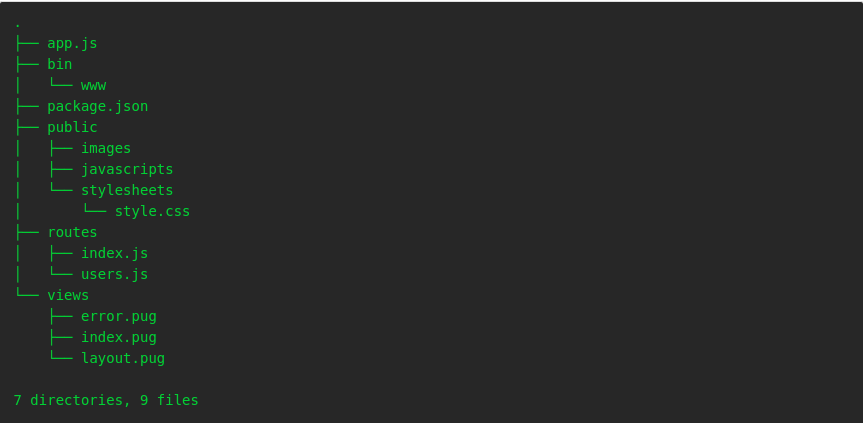
\includegraphics[width=10cm]{./Gambar/express_generator.png}
      \centering
      \caption{Tampilan direktori yang dibuat jika menjalankan express generator.}
      \label{fig:express_generator}
    \end{figure}
    
    Cara menggunakan express generator bisa dengan menjalankan command ``npx express \{nama file yang akan dibuat\}'' atau bisa dengan command ``express \{nama file yang akan dibuat\}'', maka express generator akan langsung secara otomatis membuat folder dan file-file seperti yang ada pada gambar \ref{fig:express_generator}. 
    
    \item {\textit{Routing}}\\
    Fungsi ini berguna untuk memudahkan dari web application untuk bisa menuju kepada halaman yang berbeda dengan memakai path dari alamat \textit{url} aplikasi tersebut. Cara menggunakannya adalah seperti  
\end{itemize}

\subsection{Handlebars}
\textit{Handlebars} adalah modul dari \textit{Node.js} yang membantu atas fungsi penggunaan \textit{template semantic} pada tampilan yang akan digunakan di dalam pembangunan perangkat lunak. Template semantic ini membantu pengiriman data variable dari javascript belakang ke tampilan. 

\subsection{Simple OAuth2}
Modul ini berguna untuk membantu proses otentikasi pada perangkat lunak ini yang akan melakukan otentikasi kepada aplikasi pihak ketiga lainnya. Pada \textit{simple oauth} ini dapat ditangani 3 alur untuk melakukan otentikasi yaitu:
\begin{itemize}
    \item Alur kode otorisasi\\
    Alur ini dipakai pada aplikasi yang dapat menyimpan data secara persisten. 
    \item \textit{Password Credentials}\\
    Alur ini digunakan pada saat alur sebelumnya tidak dapat dilakukan atau sedang dalam tahap pengembangan. 
    \item \textit{Client Credentials}\\
    \textit{Client} hanya bisa mendapatkan \textit{access token} dengan cara mengirimkan kredensial yang dimiliki oleh \textit{client}. 
\end{itemize}

Untuk bisa menggunakan \textit{library} ini, dibutuhkan persyaratan yaitu menggunakan \textit{Node} minimal versi 8. Jika menggunakan \textit{Node} versi 4, 5, atau 6, maka dapat menggunakan \textit{library} \textit{simple-oauth2@1.x}. Cara pemasangan library ini dengan cara menuliskan perintah pada terminal seperti: 

\begin{lstlisting}
$ npm install --save simple-oauth2
\end{lstlisting}

Saat digunakan, simple-oauth2 menerima objek yang berisi parameter yaitu: 
\begin{itemize}
    \item \textbf{\textit{client}} - objek parameter wajib yang memiliki properti: 
    \begin{itemize}
        \item \textbf{\textit{id}} - Parameter ini merupakan parameter yang dibutuhkan dan diisi dengan menggunakan \textit{client id} dari aplikasi yang sudah didaftarkan. 
        \item \textbf{\textit{secret}} - Parameter ini merupakan parameter yang dibutuhkan dan diisi dengan menggunakan \textit{client secret} dari aplikasi yang sudah didaftarkan. 
        \item \textbf{\textit{secretParamName}} - Merupakan nama parameter yang digunakan untuk mengirimkan \textit{client secret} yang memiliki nilai \textit{default} yaitu \textit{client\_secret} dari aplikasi yang sudah didaftarkan. 
        \item \textbf{\textit{idParamName}} - Merupakan nama parameter yang digunakan untuk mengirimkan \textit{client id} yang memiliki nilai \textit{default} yaitu \textit{client\_id} dari aplikasi yang sudah didaftarkan. 
    \end{itemize}
    \item \textbf{\textit{auth}} - objek parameter wajib yang memiliki properti: 
    \begin{itemize}
        \item \textbf{\textit{tokenHost}} - \textit{String} yang digunakan untuk mengatur \textit{host} untuk meminta \textit{token} dan merupakan parameter yang dibutuhkan.  
        \item \textbf{\textit{tokenPath}} - \textit{String} yang menunjukkan jalur untuk meminta \textit{access token} yang memiliki nilai \textit{default} yaitu ke \textit{/oauth/token}. 
        \item \textbf{\textit{revokePath}} - \textit{String} yang menunjukkan jalur untuk mencabut \textit{access token} yang memiliki nilai \textit{default} yaitu ke \textit{/oauth/revoke}
        \item \textbf{\textit{authorizeHost}} - \textit{String} yang digunakan untuk mengatur \textit{host} untuk meminta \textit{authorization code} dan memiliki nilai \textit{default} yaitu \textit{auth.tokenHost}. 
        \item \textbf{\textit{authorizePath}} - \textit{String} yang menunjukkan jalur untuk meminta \textit{authorization code} yang memiliki nilai \textit{default} yaitu ke \textit{/oauth/authorize}. 
    \end{itemize}
    \item \textbf{\textit{http}} - objek parameter yang bersifat opsional yang memiliki fungsi sebagai pengatur opsi \textit{global} ke \textit{internal http library} yang memiliki properti: 
    \begin{itemize}
        \item Semua opsi diperbolehkan kecuali opsi baseUrl. Memiliki nilai default yaitu headers.Accept = application/json. 
    \end{itemize}
    \item \textbf{\textit{options}} - objek parameter yang bersifat opsional yang memiliki fungsi sebagai pengatur modul yang memiliki properti: 
    \begin{itemize}
        \item \textbf{\textit{bodyFormat}} - format data yang dikirim dalam \textit{request body} saat mengirimkan \textit{request}. Nilai yang \textit{valid} untuk properti ini adalah \textit{form} atau \textit{json} dan memiliki nilai \textit{default} yaitu \textit{form}. 
        \item \textbf{\textit{authorizationMethod}} - menunjukkan metode yang dipakai untuk mengirimkan \textit{client.id/client secret} saat meminta \textit{token}. Nilai yang \textit{valid} untuk properti ini adalah \textit{header} atau \textit{body}. Jika properti ini bernilai \textit{body}, maka \textit{bodyFormat} akan dipakai untuk memformat kredensialnya. Nilai \textit{default} dari properti ini adalah \textit{header}.  
    \end{itemize}
\end{itemize}

\begin{lstlisting}
const credentials = {
  client: {
    id: <client-id>,
    secret: <client-secret>,
  },
  auth: {
    tokenHost: 'https://login.microsoftonline.com',
    authorizePath: 'common/oauth2/v2.0/authorize',
    tokenPath: 'common/oauth2/v2.0/token'
  }
};
const oauth2 = require('simple-oauth2').create(credentials);
\end{lstlisting}

\subsubsection{Alur Oauth2 yang Didukung}
\begin{itemize}
    \item Authorization Code Flow
    Authorization Code Flow menjalankan 2 langkah. Langkah pertama yaitu aplikasi akan meminta permission kepada pengguna untuk mengakses data mereka. Jika pengguna menyetujui, maka OAuth2 server akan mengirimkan authorization code kepada pengguna yang nantinya akan dilanjutkan dengan langkah kedua yaitu pengguna akan mengirimkan POST request yang berisi authorization code bersamaan dengan client secret ke oauth server untuk mendapatkan access token. 
    
    \item Password Credentials Flow
    Alur ini menggunakan username serta password untuk bisa mendapatkan access token yang dibutuhkan oleh user. Alur ini biasanya digunakan saat pengguna dengan aplikasi atau sistem operasi dari komputer sudah sangt terpercaya sehingga keamanan username dan password bisa terjaga. Cara ini biasa dipakai untuk melakukan tes aplikasi secara cepat. 
    
    \item Client Credentials Flow
    Alur ini cocok untuk pengguna yang melakukan request akses ke sumber yang dibawah kontrol dari pengguna itu sendiri. 
\end{itemize}

\subsubsection{Helpers}
\begin{itemize}
    \item Access Token object
    Saat token kadaluarsa, diperlukan refresh token untuk bisa meminta ulang access token yang baru. Simple OAuth2 menyediakan sebuah kelas AccessToken yang memiliki beragam fungsi yang salah satunya membantu mempermudah untuk meminta ulang access token saat token itu sudah kadaluarsa. Inisialisasi dari kelas ini seperti 
    
    \begin{lstlisting}
    // Sample of a JSON access token (you got it through
    previous steps)
    const tokenObject = {
      'access_token': '<access-token>',
      'refresh_token': '<refresh-token>',
      'expires_in': '7200'
    };
    \end{lstlisting}
\end{itemize}

\subsection{jsonwebtoken}
Jsonwebtoken merupakan implementasi dari JSON Web Tokens yang dikembangkan terhadap draft-ieft-oauth-json-web-token-08. Jsonwebtoken ini memiliki beberapa fungsi yaitu:
\begin{itemize}
    \item \textbf{jwt.sign(payload,secretOrPrivateKey, [options, callback])}\\
    Fungsi ini bisa berjalan secara asynchronous jika parameter callback diisi dan disediakan. Callback dipanggil dengan err atau dengan JWT. Tetapi fungsi ini juga bisa berjalan secara synchronous dan mengembalikan JsonWebToken sebagai sebuah string. 
    \item \textbf{jwt.verify(token,secretOrPrivateKey, [options, callback])}\\
    Fungsi ini bisa berjalan secara asynchronous jika parameter callback diisi dan disediakan. Callback dipanggil dengan payload yang telah di decode jika signature-nya valid dan ada parameter seperti kadaluarsa yang bersifat opsional, audiens, atau penerbit akan menjadi valid. Jika tidak, maka akan menimbulkan error. Fungsi ini juga bisa berjalan secara synchronous jika tidak ada callback yang diisi. 
    \item \textbf{jwt.decode(token, [options])}\\
    Fungsi ini berjalan secara synchronous dan mengembalikan payload yang sudah di decode tanpa memverifikasi signature yang ada valid atau tidak. 
\end{itemize}

\subsection{Isomorphic Fetch}
\textit{Isomorphic Fetch} adalah sebuah \textit{polyfill} \textit{window.fetch} untuk digunakan di \textit{node} dan \textit{browserify}. \textit{Polyfill} ini memungkinkan \textit{window.fetch} untuk \textit{javascript engine} yang tidak mendukungnya secara \textit{native}. 

\subsection{Microsoft Graph Client Library}
Microsoft Graph Client Library adalah sebuah library yang disediakan oleh Microsoft untuk perangkat lunak yang akan menggunakan API ke Microsoft bisa lebih mudah. Library ini hanya sebagai pembungkus dari semua fungsi API yang disediakan oleh Microsoft. Untuk bisa memakainya, maka harus menginisialisasi terlebih dahulu sebuah objek inisialisasi dari library ini dengan menggunakan access token yang didapat saat melakukan request awal. Setelah melakukan inisialisasi, maka setiap API dapat diakses dengan menjalankan kode seperti:

\begin{lstlisting}
const result = await client.api(`/me/events`).select('subject,start,end').orderby('start/dateTime DESC').get();
\end{lstlisting}

Api diatas diisi dengan fungsi yang akan dipanggil lalu select diatas diisi dengan data yang akan diambil. Orderby digunakan untuk jika data ingin diurutkan berdasarkan urutan tertentu.

\subsection{Slack Web API}
Sama seperti Microsoft Graph Client Library, Slack Web API ini juga adalah library yang membungkus method-methid yang disediakan oleh Slack agar untuk mengakses method bisa lebih mudah. Cara menggunakannya adalah dengan menginisialisasi terlebih dahulu library yang akan dipakai sebagai kelas yang akan dipakai, lalu menginisialisasi kelas ke sebuah variable yang diisikan dengan parameter slack access token yang didapat dari request. Setelah itu, jalankan variable tersebut dengan memanggil scope yang dipakai seperti contoh pada code:

\begin{lstlisting}
const web = new WebClient(slack_access_token);

  const result = await web.users.profile.set({
    "profile":{
        "status_text": "In A Meeting",
        "status_emoji": ":no_entry:"
      }
  });
\end{lstlisting}

Untuk setiap scope yang dipakai akan memerlukan request body yang berbeda-beda. Untuk mengetahui request body yang diperlukan, dapat dilihat pada \url{https://api.slack.com/methods}. 

\section{Heroku}
Heroku adalah \textit{cloud platform} yang menampung program agar bisa dibangun, dan dijalankan di \textit{cloud}.\cite{heroku} Heroku mendukung beberapa bahasa pemrograman yaitu: Ruby, Node.js, Java, Python, Clojure, Scala, Go, dan PHP. 
\subsection{Dyno}
Dyno adalah sebuah wadah berbasis Unix yang disediakan oleh Heroku. Dyno disini dikategorikan ke 3 jenis dyno yaitu:
\begin{itemize}
    \item Web Dyno \\ 
    Web dyno adalah dyno yang berjalan pada tipe proses web. Web dyno adalah satu-satunya dyno yang bisa menerima HTTP dari router heroku. 
    \item Worker Dyno \\ 
    Worker dyno adalah dyno yang berjalan selain pada tipe proses web. Worker dyno biasa digunakan untuk pekerjaan pada latar belakang, sistem antrian, dan pekerjaan berjangka waktu tertentu. 
    \item One-off Dyno \\ 
    One-off dyno adalah dyno yang bersifat sementara dan contoh penggunaannya adalah seperti saat migrasi basis data. Dyno ini dijalankan menggunakan command shell. 
\end{itemize}
Heroku menyediakan beberapa paket dyno yang mempengaruhi karakteristik dan juga cara kerja dyno seperti:
\begin{itemize}
    \item Free \\ 
    Pada paket ini, jumlah dyno yang didapat untuk setiap proccess type adalah 1 serta adanya batasan dyno hours yaitu sebanyak 550 jam untuk akun yang belum terverifikasi dan 1000 jam untuk akun yang sudah terverifikasi. Dyno akan memasuki kondisi sleep jika web dyno sedang tidak aktif selama lebih dari 30 menit. Dyno akan kembali lagi aktif ketika ada arus yang masuk ke HTTP tetapi ada keterlambatan untuk memproses arus tersebut.  
    \item Hobby \\ 
    Jumlah dyno yang didapat untuk setiap proccess type adalah 1. Jumlah dyno hours di dalam paket ini tidak dibatasi tetapi setiap dyno hours yang dipakai akan dikenakan biaya sebesar \$7 per jam per bulannya.  
    \item Standard \\
    Jumlah dyno yang didapat untuk setiap proccess type adalah sebanyak 10. Jumlah dyno yang bisa dijalankan secara bersamaan adalah sebanyak 100 pada satu aplikasi. Harga dari dyno hours berkisar antara \$25 sampai \$500. 
    \item Performance \\
    Jumlah dyno yang didapat untuk setiap proccess type adalah sebanyak 10. Jumlah dyno yang bisa dijalankan secara bersamaan adalah sebanyak 100 pada satu aplikasi. Harga dari dyno hours berkisar antara \$25 sampai \$500. Perbedaan dari paket standard dengan paket performance adalah paket ini bersifat dedicated. 
\end{itemize}

Pada heroku terdapat banyak fitur-fitur penyokong untuk menjalankan aplikasi seperti basis data, sistem antrean, layanan email, dan lain-lain yang disebut dengan \textit{add-ons}. Daftar dari \textit{add-ons} yang tersedia untuk Heroku dapat dilihat pada situs web \textit{Elements Marketplace} (\url{https://elements.heroku.com/addons}) Beberapa contoh \textit{add-ons} yang tersedia di \textit{heroku} antara lain:

\subsection{Heroku Scheduler}
Scheduler adalah add-ons gratis yang bertugas untuk mengatur jalannya pekerjaan dalam aplikasi secara berkala sesuai dengan interval yang ditentukan oleh pengguna. Tugas heroku scheduler lebih mirip dengan cara kerja cron di server tradisional. Melalui scheduler, pekerjaan dimungkinkan untuk dijalankan setiap 10 menit sekali, setiap jam, setiap hari, atau pada waktu yang ditentukan. Saat dijalankan, job ini akan berjalan sebagai one-off dynos dan akan muncul di dalam logs sebagai dyno seperti scheduler.X. Cara memasang add-ons ini melalui command shell adalah dengan cara:
\begin{lstlisting}
\$ heroku addons:create scheduler:standard
\end{lstlisting}
Scheduler akan menjalankan one-off dynos yang akan dihitung sebagai penggunaan dari pengguna pada bulan itu. Dyno-hours yang dihitung akan sama seperti saat menjalankan aplikasi atau dari dynos yang berskala. Untuk pemakaian dari dyno-hours dapat pengguna lihat pada bagian tagihan pada tab ``\textit{Manage account}''. 

\subsection{Heroku Postgres}
Heroku Postgres adalah layanan basis data SQL yang dikelola dan disediakan langsung oleh Heroku. Basis data Heroku Postgres dapat diakses dengan menggunakan semua bahasa pemrograman dengan driver PostgreSQL termasuk seluruh bahasa pemrograman yang didukung di Heroku. Untuk cara penggunaannya di dalam bahasa Node.js, maka dibutuhkan langkah-langkah yaitu 
\begin{itemize}
    \item Melakukan pemasangan modul pg sebagai dependency dengan cara menjalankan command line seperti:
    \begin{lstlisting}
    $ npm install pg 
    \end{lstlisting}
    \item Melakukan koneksi ke url dari basis data yang disediakan oleh Heroku saat perangkat lunak dijalankan. Contoh dari kode programnya seperti:
    \begin{lstlisting}
    const { Client } = require('pg');

    const client = new Client({
      connectionString: database_url,
      ssl: true,
    });
    
    client.connect();
    
    client.query('SELECT table_schema,table_name FROM
    information_schema.tables;', (err, res) => {
      if (err) throw err;
      for (let row of res.rows) {
        console.log(JSON.stringify(row));
      }
      client.end();
    });
    \end{lstlisting}
\end{itemize}
